\chapter{The distance ladder} \label{ch:distance_ladder}

%\section{Distance ladder}
Although many Type Ia supernova have been studied in detail, with photometric time series and more-costly spectra, that information cannot on its own tell us how luminous the explosions are.  Furthermore, they are rare enough and none are close enough for direct geometric measurements of their distances.  We need to calibrate them with another type of object, usually Cepheid-type variable stars.  Some Cepheids are near enough to us to measure their distance geometrically via parallax, using the Earth's orbit around the Sun, the size of which is precisely known from radar ranging to the planets and measuring their orbits and periods.  We know those Cepheids' luminosities by comparing their measured brightness to that distance.  By extrapolating those results to Cepheids that are too far for parallax but bright enough to see in intermediate-distance galaxies that also hosted Type Ia supernovae, we can determine the distances to those galaxies and calibrate the luminosities of the Type Ia supernovae as a class.  That allows us to use the larger number of even further-out supernovae to measure the normalization of the distance--redshift relation, $1/H_0$, not just the shape.

% Using nomeclature of 2025arXiv251023823H
Thus to build a ``ladder'' to the distant Universe, we use parallax measurements (rung 1) of the Milky Way Cepheids to anchor the luminosity calibration for the Cepheids.  Then we use extragalactic Cepheid brightnesses (rung 2) as a primary distance indicator to determine distances to the galactic hosts of supernovae and calibrate their luminosities.  We then use the supernovae as secondary distance indicators (rung 3), reaching well out into the Hubble flow \citep[][]{2025arXiv251023823H}.  

At the end of the chapter, we'll also discuss some alternative objects and methods for measuring distance, including other types of supernovae and stars and even gravitational waves.
 

\section{Cepheid variable stars}

\begin{table}[t]
  \begin{tabular}{lllll}
    Property & Classical Cepheid \\
    \hline
    \\
    \\
    \hline
  \end{tabular}
  \caption{\textcolor{purple}{Placeholder table with basic properties of variable stars discussed, Classical Cepheids, Type II Cepheids, RR Lyrae stars, Mira Variables.}}
\end{table}


Cepheid stars have a periodic variability and the period is strongly correlated to the overall luminosity.\footnote{Famously noted by Henrietta Leavitt in 1912.}  They are common enough in the Milky Way that we can calibrate the period--luminosity relation via geometric parallax with HST, Hipparcos, and Gaia data.  That makes them useful distance indicators.  They are a heterogeneous grouping of a few different types of objects.

% This OGLE webpage is great: https://ogle.astrouw.edu.pl/atlas/classical_Cepheids.html

Classical Cepheid stars (also called Population I Cepheids, Type I Cepheids, and Delta Cepheid variables) are young, metal-rich, population I stars (from the current generation of star formation).  They are between roughly 4--20 $M_\odot$, with the range skewing higher for lower  metallicity.  They are mostly former spectral-type-B stars that have evolved off the main sequence and have luminosities much greater than the Sun, about $10^3$--$5\times 10^4$ $L_\odot$.  Thus they can be seen individually in many external galaxies.  As they burn shell hydrogen, or burn shell or core helium, they cross into or repeatedly loop through the instability strip of the Hertzspring-Russell luminosity--surface temperature diagram, where stars are subject to variability and pulsations.  Classical Cepheids execute radial pulsations that are a few days to a few weeks in duration.  The class is named for Delta Cephei, fourth-brightest star in the Constellation Cephus, an early star of this class to be characterized and one for which the parallax distance is the best known. The North Star, Polaris, is another prominent example.


\begin{figure}[!t]
    \begin{minipage}[t]{0.5\textwidth}
      \begin{center}
        Classical Cepheids \\
        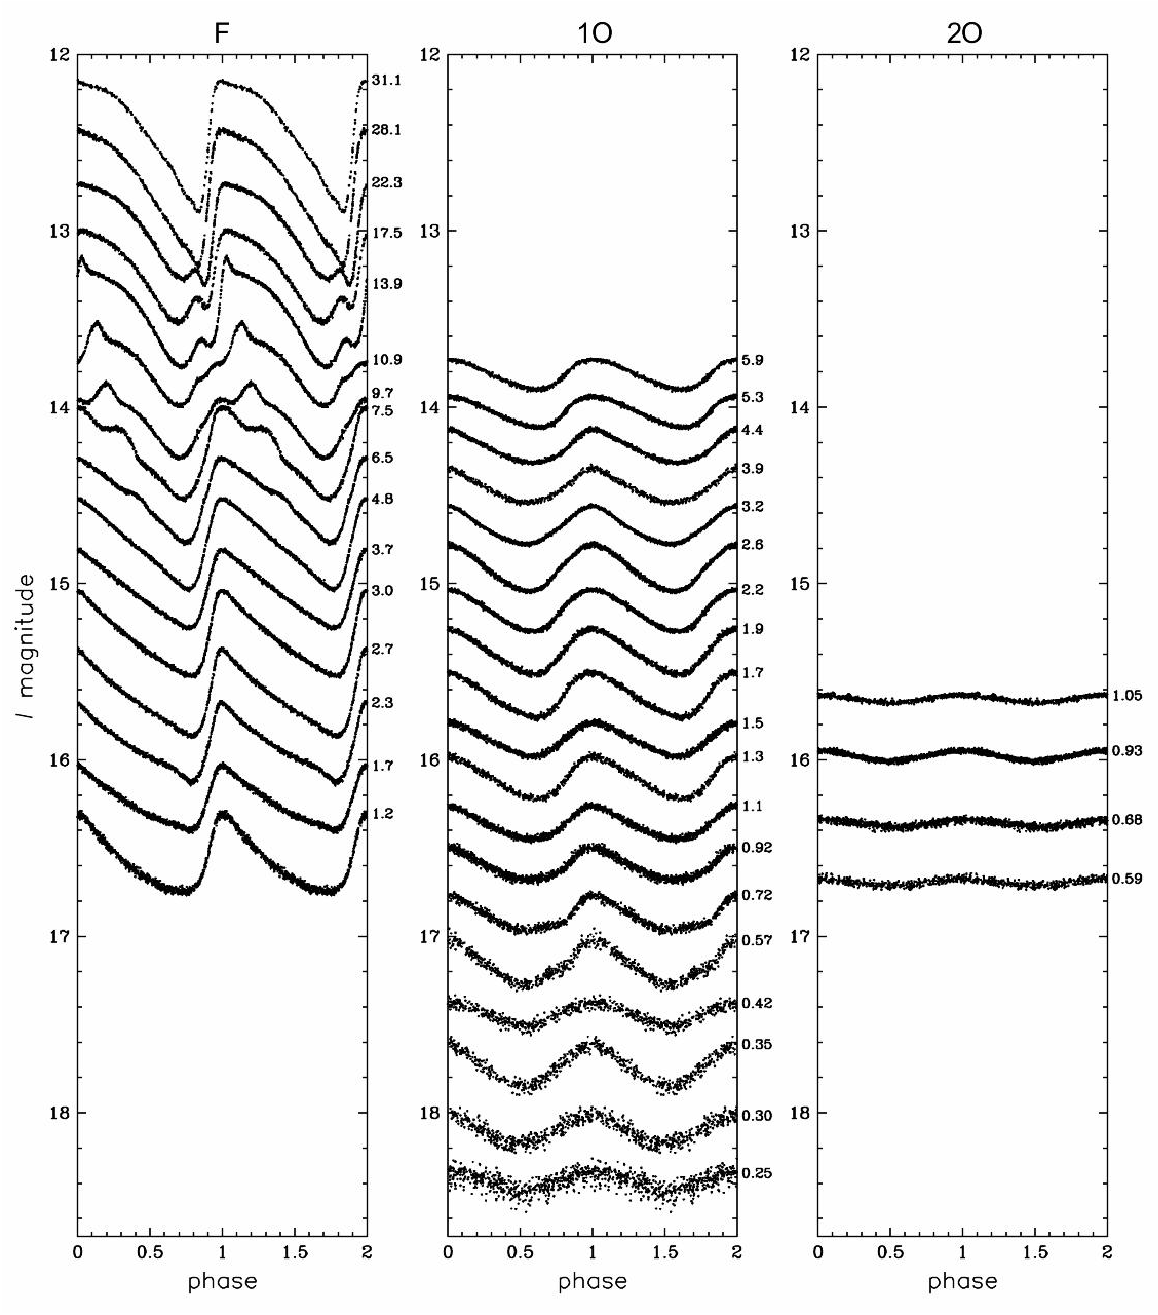
\includegraphics[width=\textwidth]{figs/standard_candles/OGLE_Cepheid-classical-lightcurves-crop.pdf}
        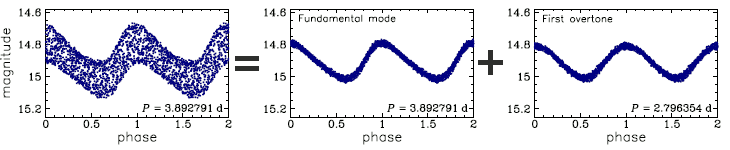
\includegraphics[width=\textwidth]{figs/standard_candles/OGLE-LMC-CEP-0832.png}
      \end{center}
    \end{minipage}
    \begin{minipage}[t]{0.5\textwidth}
      \begin{center}
        Type II Cepheids \\
      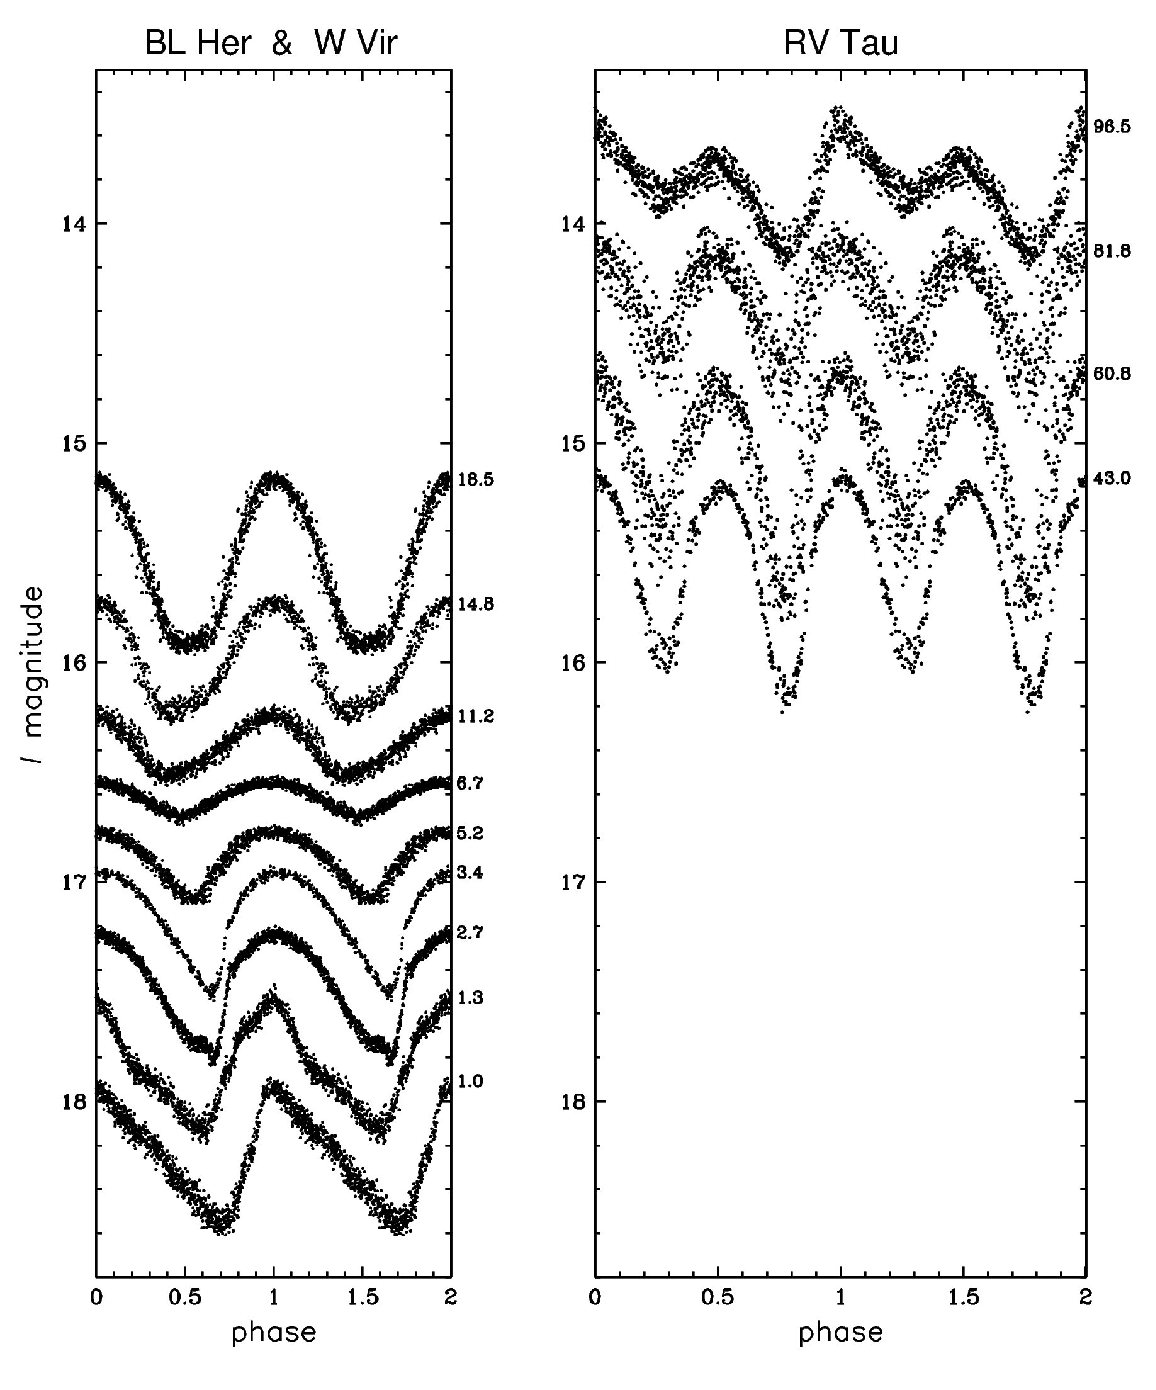
\includegraphics[width=\textwidth]{figs/standard_candles/OGLE_Cepheid-type2-lightcurves-crop.pdf}
      \end{center}
      \end{minipage}
  \caption{Cepheid light curves, folded in phase to match the oscillation period.  All stars are at the same distance in the LMC.  Classical Cepheids are to the left \citep[][]{2008AcA....58..163S}, and among them, top left-to-right, are those pulsing at the fundamental mode, the first overtone, and the second overtone.  The left vertical axis shows the I band magnitude.  Each right axis is labeled by the period of the star in days.  Bottom left, a classical Cepheid star that is excited in both the fundamental mode and the first overtone.  Type II Cepheids are to the right  \citep{2008AcA....58..293S}, divided at 4-day and 20-day periods into three subclasses.  Long-period RV Tau stars have been phased with double the formal periods to illustrate alternating bright and dim minima.}  \label{fig:cepheid_light_curves}
\end{figure}

Type II Cepheid stars (also called Population II Cepheids)  are such a different class of objects that they perhaps ought to have a different name.  They are old, metal-poor, low-mass population II stars from a previous generation of star formation.  These stars may be $0.5$--$1$ $M_\odot$ or less.   Type II Cepheids themselves are a heterogeneous group, with short-, medium-, and long- period subclasses at different stages of evolution off the main sequence between red giant and post-AGB phase.
%Some show alternating shallow and deep minima.
For a given period, Type II are fainter than classical cepheids by a factor of 4--5, but still much more luminous than the Sun.  Early cosmological studies mistook Type II Cepheids in other galaxies for classical Cepheids, making roughly a factor of two error in the distance and the Hubble constant.  Type II Cepheids have a period--luminosity relationship that is less metallicity dependent than for classical Cepheids.

\begin{figure}[!t]
  \begin{minipage}[t]{0.5\textwidth}
    \begin{center}
      Classical Cepheids \\
      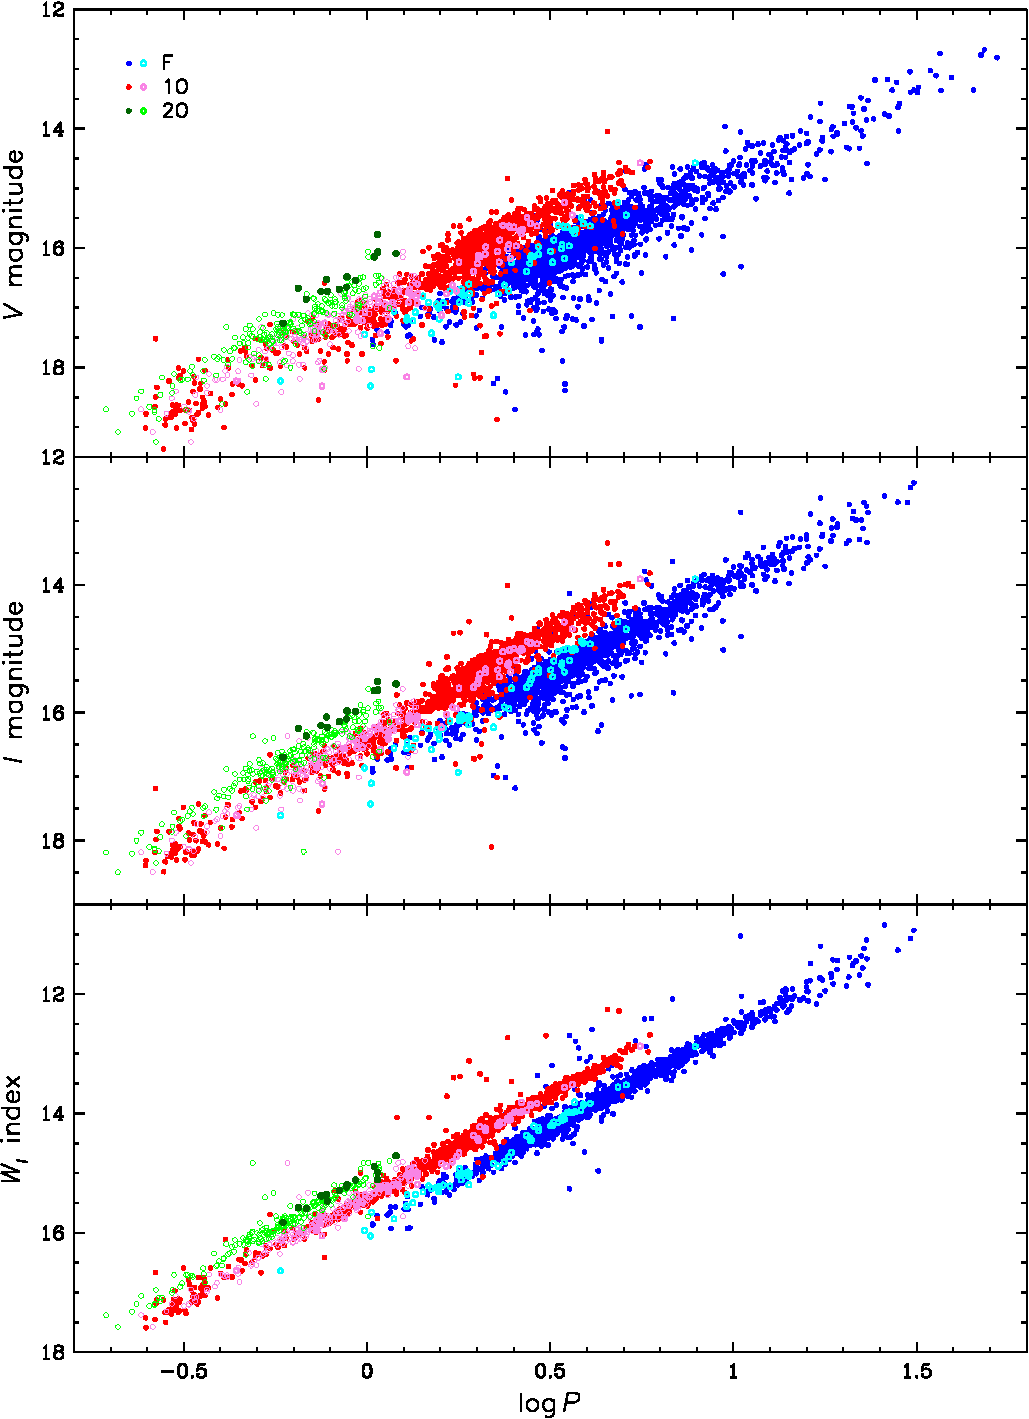
\includegraphics[width=\textwidth]{figs/standard_candles/OGLE_Cepheid-classical-period-luminosity-crop.pdf}
    \end{center}
  \end{minipage}
  \begin{minipage}[t]{0.5\textwidth}
    \begin{center}
      Type II Cepheids \\
      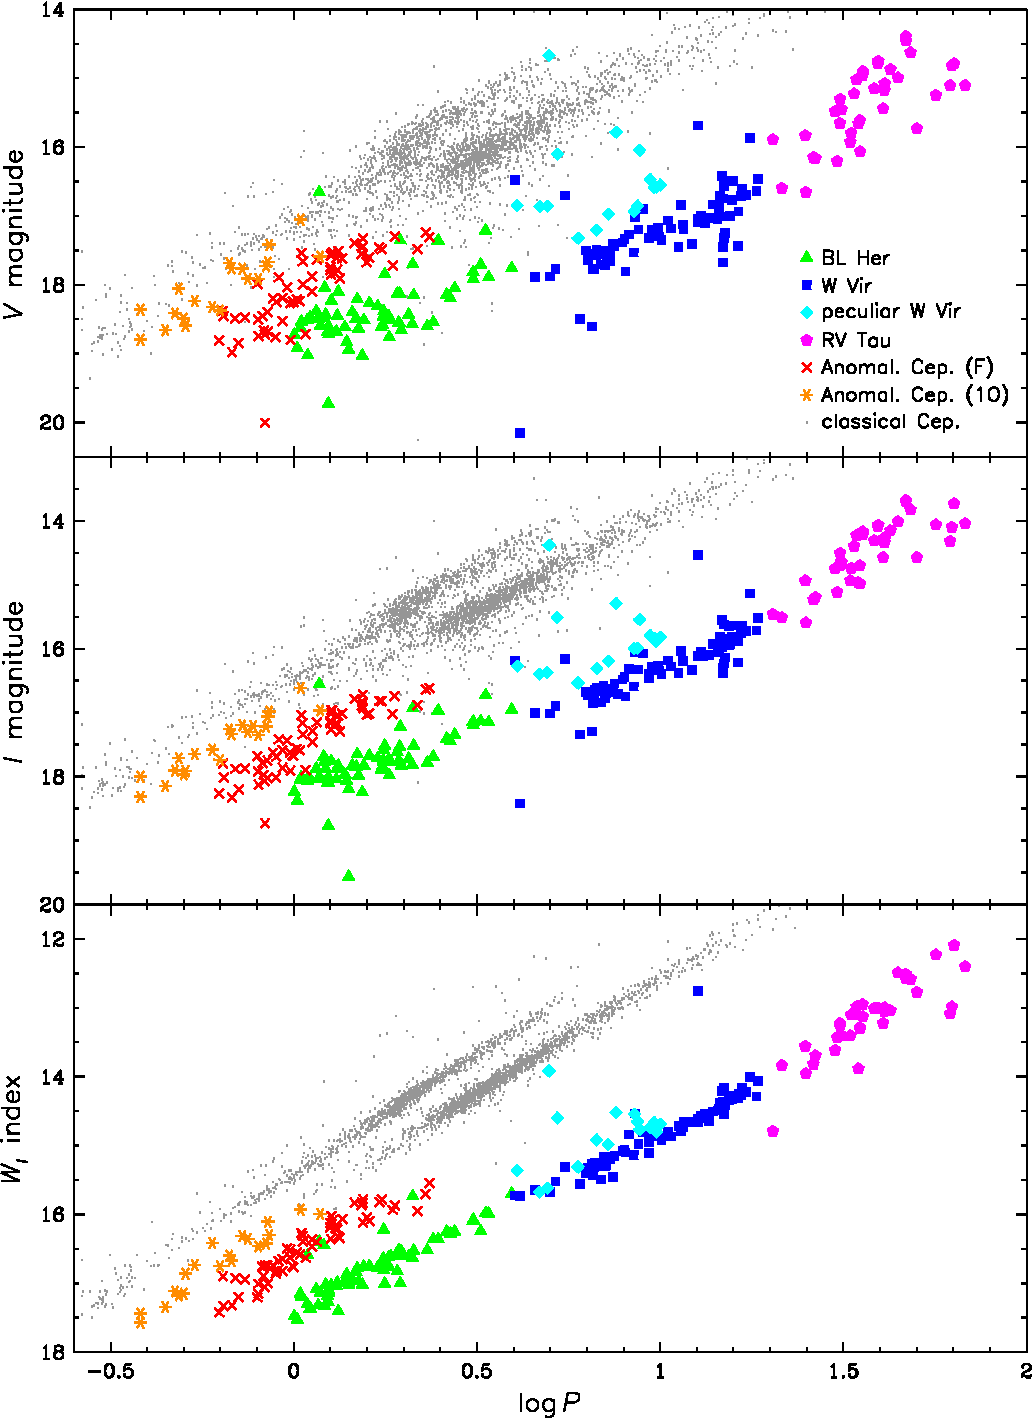
\includegraphics[width=\textwidth]{figs/standard_candles/OGLE_Cepheid-Type2_period_luminosity-crop.pdf}
    \end{center}
  \end{minipage}
  \caption{Period--luminosity relationships for Cepheid variable stars, all in the LMC with roughly the same distance  from \citep[][]{2008AcA....58..163S,2008AcA....58..293S}.  The horizontal axis shows the log-base-10 of the pulsation period in days.   Periods range from less than a day to about 90 days.  Vertical axes show V band magnitude, I band magnitude, and their combination in the Wesenheit index, which shows less scatter.  Left, classical Cepheids show the separate relationship for stars oscillating is the fundametal or overtone modes.  Solid dots are single-mode oscillators and empty dots are two-mode oscillators, with two points plotted per star.  Right, type II Cepheids of several varieties (colored symbols) are lower in brightness than classical cepheids (gray dots)} \label{fig:cepheid_period_luminosity}
\end{figure}

For both types of stars, the pulsation mechanism relates to opacity.  In a normal star, as temperature and pressure increase, the opacity decreases, allowing more light energy to escape and maintaining an equilibrium. In a star where the opacity increases with temperature, an increase in density raises the temperature, which traps more light, raising the temperature further.  The pressure builds up, causing the star to swell up in size.  The falling density lowers the temperature.  Opacity decreases and light begins to escape more easily, lowering the temperature and opacity more, and the pressure decreases.  The loss of pressure causes the star to shrink and the process repeats.  In both classes of Cepheid stars, a layer of {singly-ionized helium} is responsible for the opacity changes.  Some other types of pulsating stars have the same basic mechanism,  RR Lyrae stars for instance, which are similar to Type II Cepheids but are horizontal branch stars on an earlier transit of the instability strip.

The star acts like a damped, driven oscillator: when the frequency of the opacity on-off cycle matches a resonant frequency of the Cepheid, it can drive large-amplitude pulsations.  The fractional change in radius $\Delta R/R$ can be 5--15 percent in classical Cepheids and up to 30 percent for some types of Type II Cepheids.  Longer periods correlate with larger amplitudes.  The increase in radius causes an increase the luminosity that we observed.  The damping is caused by loss of energy due to heat transport (``heat leak'') or turbulent viscous dissipation, depending on the type of Cepheid and the location within the star.

In classical Cepheids, when the star's fundamental frequency is excited, typically the light curves are asymmetric, with a faster rise than fall.  See Figure~\ref{fig:cepheid_light_curves}, left panels.\footnote{In fundamental mode Cepheids, between about six and twenty-five day periods, there is a bump in the light curve caused by a 1:2 resonance betweeen the fundamental and second overtone.  The phase location of the bump changes a regular way, called the Hertzsprung progression.}  The bulk of the expansion is in the outer layers, but the whole star expands and contracts together.  When the first overtone is the dominant one excited, the outer layer expands while the inner layers contract (and vice versa) and there is a single, stationary, node radius.  When the second overtone is excited, there are three alternating layers expanding and contracting and two node radii.  The overtone pulsations are more sinusoidal and smaller in amplitude.  Rarely, two or three modes are excited by similar amounts.  With long-duration photometric data on the star, detailed Fourier analysis of the light curves can reveal which modes are excited.  Light curves can also be modified in binary systems where the star may be eclipsed or tidally distorted into an ellipsoid.  These will imprint the binary period into the light curve.

Light curves of Type II Cephieds are more complicated, varying by subtype and can be glitchy from flashes of helium fusion.  Long-period Type II Cepheids show alternating deep and dim minima.

The physical processes of pulsation occur with a longer period in a physically larger star, which are also more luminous.  Unfortunately, there is not a physical model of the period-luminosity relationship that provides the precision necessary for fitting distances, so the period--luminosity relationship must be calibrated emprically.  Figure \ref{fig:cepheid_period_luminosity} shows the luminosity versus period for a large number of Cepheid stars, all at a similar distance in the LMC.\footnote{The LMC distance is $49.59 \pm 0.09$ (statistical) $\pm 0.54$ (systematic) kpc by the detached ecliping binaries method \citep[][]{2019Natur.567..200P} discussed at the end of the chapter.}
% $49.97 \pm 0.19$ (statistical) $\pm 1.11$ (systematic) kpc \citep{2013Natur.495...76P}).
Each different sub-category of Cepheid has its own period--luminosity relationship.  These relationships show color dependence, and the scatter is minimized using the Wesenheit index between the infrared- and visible-band magnitudes, $W_I$ = $m_I - 1.55(m_V - m_I)$.

%are luminous (absolute magnitude $M \sim -1$ to $M \sim -5$ versus $M = +4.83$ for the Sun) and
For Cepheids near enough to get a parallax measurement, we can establish the period relationship for the absolute magnitude or luminosity.  The numbers of  objects that anchor our cosmological distance measurements is not large.  As of 2025, fewer than \textcolor{red}{100} Cepheids have parallax measurements in the Milky way or magellanic clouds.  The megamaser galaxy NGC 4258 (more on this later), which allows a (rare) geometric measurement of the angular diameter distance %($D_A = 7.60 \pm 0.17 \pm 0.15$ Mpc)
to the central keplerian disk, helps with the calibration of Cepheids because that galaxy has a broader range of metallicities that overlaps both with the Milky Way and other galaxies.\footnote{The Milky Way has a higher than average metallicity and a strong radial metallicity gradient compared to other galaxies, perhaps indicating that the Milky Way suffered fewer than average disruptive galaxy mergers in its history.}




% Maximum distance that we can see a cepheid?



\section{Alternative rungs for the distance ladder}
There are a multitude of measurements that use the properties of some class of objects as distance indicators.  We will provide just a sampling of alternatives to the current standard of cepheid-to-Type Ia supernovae.  In the following chapters, we will also see how correlations in the density field can serve as a standard ruler, providing another avenue to measure distances.


\begin{figure}[!t]
  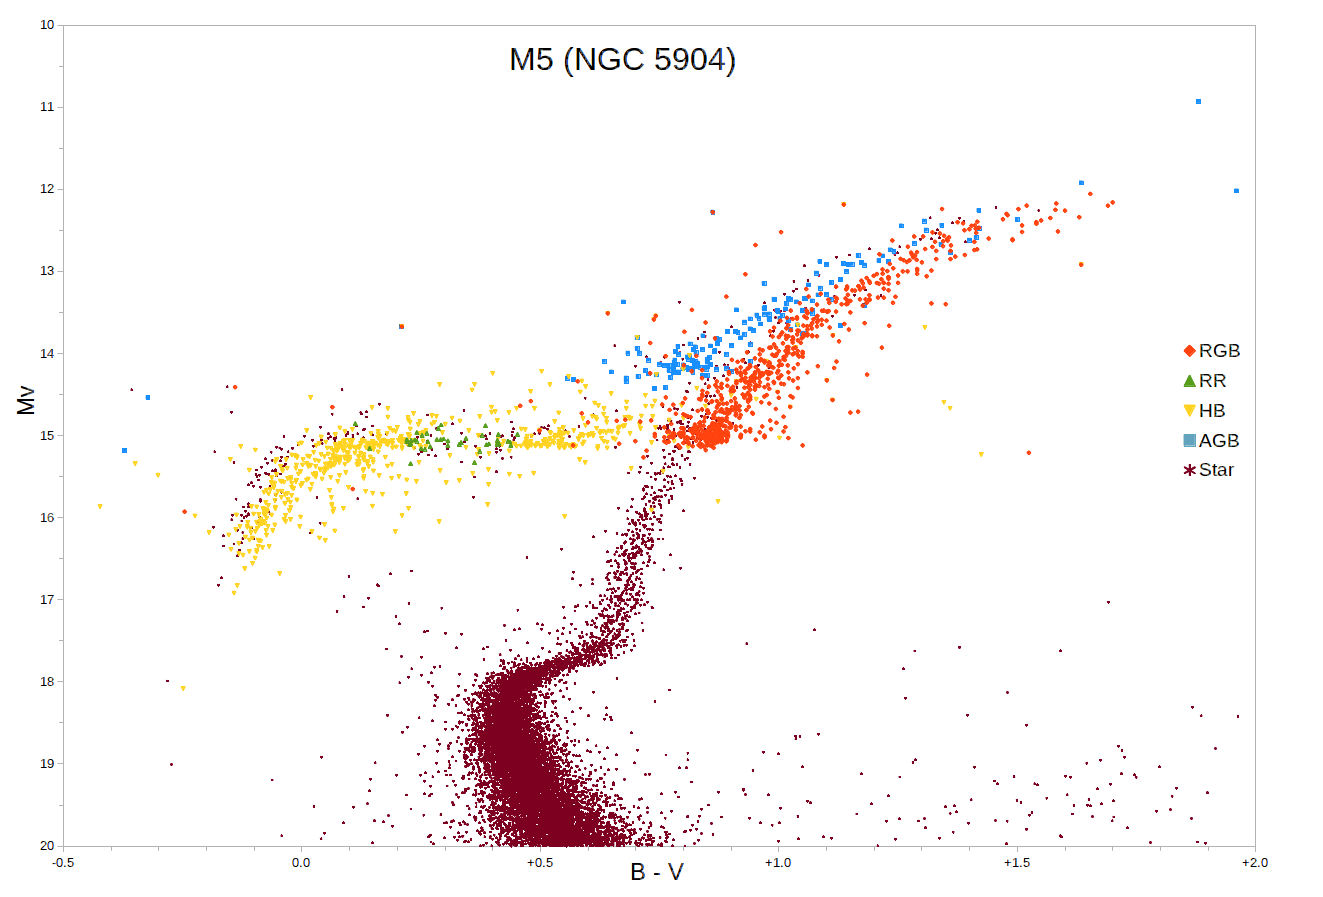
\includegraphics[width=\textwidth]{figs/standard_candles/M5_colour_magnitude_diagram.png}
  % https://commons.wikimedia.org/wiki/File:M5_colour_magnitude_diagram.png
  \caption{Color--magnitude diagram for stars in the globular cluster Messier 5, showing a snapshot of the stages of stellar evolution for stars of differing mass.  At the bottom of the diagram, the main sequence (dark red) comes up from the bottom and turns sharply right where the more massive stars have evolve off the main sequence into the subgiant branch (also dark red) and into the red giant branch (RGB, dark red to red).  Even more massive stars have finished the red giant phase and are horizontal branch stars (yellow), including RR Lyrae stars (green) in the instability strip.  Cepheids, which are brighter, would appear above the RR Lyrae stars if present.  Even more massive stars have further evolved into asymptotic giant branch (AGB) stars.}
\end{figure}

\subsection{Geometric distance anchors}

There are other direct distance anchors, rather than parallax, to base the first rung of the distance ladder on, but they don't yet match Cepheid parallaxes in statistical precision.  

\paragraph{Detached eclipsing binaries.}  For eclipsing binary stars, where the plane of the orbit is edge-on to the line of sight, photometry of the light curve can reveal if the eclipse is partial or total and whether the binaries are detached or in contact.  Doppler shifts of the spectral lines reveal the velocity of the orbit, so the duration of the eclipse can reveal the radii of the stars.  With star's surface area and the spectral energy distribution (largely determined by the blackbody emission of the effective temperature) we can compute the luminosity (roughly $L = 4\pi R^2 \sigma T_{\rm eff}^4$), compare it to the brightness in several bands, and determine the luminosity distance.  As mentioned before, the LMC distance has been anchored with eclipsing binaries, which can be used to calibrate the Cepheids therein.

\paragraph{Masers.} A handful of galaxies have been discovered that contain masers in the accretion disk at the central black hole.  An astrophysical maser is like a natural microwave laser, a two-level system with an inverted population that generates intense stimulated  monochromatic line emission, but without the resonant cavity of the fabricated device.  The prototypical disk megamaser galaxy is NGC 4258, but there are a half dozen more.

A particular accretion disk may contain some hundreds of maser spots, distributed in several clumps within a couple of parsecs, or a couple of milli-arcseconds, of the black hole.  Very-long baseline interferometry, correlating a global network of radio telescopes, can measure the spot positions to several $\mu$as accuracy.   Single dish and interferometric observations can measure line velocities and over the course of a few years, the line-of-sight spot accelerations to fractions of a km/s/yr.  The centripetal acceleration in the plane of the Keplerian disk, $a_c = G M_{\rm BH}/r^2 $, can be translated to line-of-sight acceleration with the disk's inclination angle, and the physical radius can be translated to the sky position via the angular diameter distance, the quantity we would like to determine.

The actual modeling is somewhat more complex, with fitting parameters for the galaxy distance, the black hole mass and center, disk inclination and position angle, warping of the disks to second order in the radius (in both the inclination- and position-angle-directions), and the ellipticity and orientation of the major axis with direction.  In addition, each maser spot gets two parameters for its position in the disk.  
A few of these systems are distant enough to be in the Hubble flow, and their precisions make them really excellent distance indicators, but overall they are rare and the measurements and modeling is involved.


\paragraph{Type II-P supernovae (SNe II-P).}  Type II supernovae (with hydrogen lines) are an alternative to type Ia supernova.  The II-P subclass has plateau in the light curve where the luminosity is roughly constant.  The supernova explosion ionizes the star's large and intact hydrogen envelope, which cools and recombines from the outside in.  The ionization energy of hydrogen is well-known, so this recombination occurs at a roughly steady temperature.  The recombination front defines the photosphere.  The large envelope also makes the supernova more symmetric.

The distance estimate methods for II-Ps, going by names like the Expanding Photosphere Method,  Standardized Candle Method, or Photospheric Magnitude Method, are variations on a single concept.  Spectroscopy can provide the velocity of the photosphere.  The expansion at this phase is homologous: the gas is freely coasting under negligable gravitational and pressure forces and so each gas shell has constant radial velocity---faster on the outside, slower on the inside, and proportional to radius at any given time.  The particular shell in the photosphere that we measure the velocity of changes as the outward-moving gas shells successively recombine.  Shell constant velocities can be compared to give the time of explosion and integrated to yield a physical size.  The surface area and the emission model yields the luminosity.  This is compared to the measured brightness to give the luminosity distance.  Exercise \ref{ex:SNII-p} at the end of the chapter explores this strategy in some detail.

The complication for this method is that the there is significant scattering of the light in the supernova's atmosphere.  The emission is not a simple black body, but requires non-equilibrium radiation transport modeling to compute the ``dilution'' efficiency factor of the emission, which depends on the density profile, the metallicity, and the velocity broadening of spectral lines.  While the expanding photosphere method is purely physical and geometric, some of the variants of the method employ empirical correlations between expansion velocity and plateau luminosity at different epochs.  This partially alleviates the need for atmospheric modeling, but requires a distance calibration; in that case the II-P supernovae serve as secondary distance indicators rather than anchors.


%The typical distance precision is now about 15 percent per object.



\paragraph{Gravitational wave standard sirens.} Beyond the electromagnetic sources that we have been considering, gravitational-wave emitters also show great promise to measure cosmological distances, although there are significant challenges.

In a compact binary with a quasi-circular inspiral, the gravitational wave strain (fractional stretching of length $\Delta \ell/\ell$) in the two polarizations depends on the luminosity distance as \citep{2005ApJ...629...15H,2007gwte.book.....M},
\begin{eqnarray}
  h_+(t) &=& \frac{4[(1+z) {\cal M}_c ]^{5/3} [\pi f(t)]^{2/3}}{D_L(z)} \frac{ 1 + \cos^2(\iota) }{2} \cos(\Phi(t)) \\
  h_\times(t) &=& \frac{4[(1+z) {\cal M}_c ]^{5/3} [\pi f(t)]^{2/3}}{D_L(z)} \cos(\iota) \sin(\Phi(t)), \label{eqn:GW_distance_measure}
\end{eqnarray}
where the ``chirp mass'' combination of the two masses in the binary is\footnote{The combination $ {\cal M}_z = (1+z) {\cal M}_c$ is the observable, detector-frame, redshifted chirp mass.}
\begin{equation}
 {\cal M}_c = \frac{(m_1 m_2)^{3/5}}{(m_1 + m_2)^{1/5}},
\end{equation}
the observed frequency is $f$, the inclination angle $\iota$ is the angle between the line of sight and the system's orbital angular momentum ($\iota=0^\circ$ is face-on, $\iota = 90^\circ$ is edge-on), and the phase of the binary is $\Phi(t) = 2\pi  \int  f(t)  dt$.\footnote{The phase over long periods is not simply $2\pi ft$ because of the inspiral and the non-constant frequency.}
The evolution of the phase and frequency depends on the masses and spins of the members and the chirp mass.  For non-spinning black holes, the (redshifted) chirp mass alone determines the derivative of the frequency and the inspiral rate and is well determined by measuring the waveform.

A single gravitational wave interferometer is sensitive to a projection of the two polarizations, providing a noisy measurement of 
\begin{equation}
  h = F_+(\theta,\phi,\psi) h_+(t) + F_\times(\theta,\phi,\psi) h_\times(t),
\end{equation}
where $F_{+,\times}$ is the angular instrumental response (or beam) to a polarization at that sky angle $(\theta,\phi)$ and polarization reference angle ($\psi$).  Gravitational distance measurements suffer from significant inclination degeneracy, and are unable to distinguish a nearby, edge-on binary from a distant, face-on one.  Additional interferometers in different orientations improve the solution for inclination.   Localization is also a significant problem.  The graviational waveform does not tell us the redshift.  There is a degeneracy between a low-redshift, low-mass binary and high-redshift, high-mass binary.  We therefore need to identify the host galaxy of the binary so that we can measure its redshift.  For current interferometers, the localization is only a few square degrees at best, so we need to find some visual transient counterpart of an inspiral and merger to localize the host.  Additional interferometers also help with localization.  Neutron star mergers (''kilonova'') therefore make especially good targets because of the afterglow, while black hole--black hole mergers may not have much of a visible counterpart.

Even for black holes, if the sky localization is sufficiently narrow, the statistical combination of a large number of mergers can self-calibrate the method.  A single merger with the inclination resolved yields a precise $D_L$; this will allow several discrete distance--redshift pairs, one per candidate host galaxy within the localization.  In that case, we will know the distance but not the redshift, only several possibilities, the opposite problem to our other distance methods.  Considering a large number of mergers, we are limited to a cosmological model that provides a distance--redshift relation compatible with each merger. We can account for the possibility of out-of-catalog galaxies with a completeness correction, adding a smooth probability distribution in redshift to account for galaxies we may have missed.  In such statistical analyses, we must also account for the selection bias that we sample GW mergers down to some loudness limit, and more massive systems can be detected to greater distance (an example of ``Malmquist'' bias).

Eccentric orbits add harmonics to the waveform that can help to break degeneracies, but the late stages of the inspiral serve to circularize the orbit.  The non-linear memory effect, the slight, but permanent, adjustment to our local spacetime (an accumulated overall $\Delta \ell/\ell$) caused by the passing of a gravitational wave pulse has a distinct dependence on inclination angle.  The LIGO, Virgo, and KAGRA observatories are not sensitive enough to see the memory effect, but LISA and the Einstein telescope would be able to use it to break the inclination degeneracy.

Importantly, gravitational wave detectors are sensitive to the strain directly, so the signal declines as the inverse first power of the luminosity distance in Equation (\ref{eqn:GW_distance_measure}), rather than the inverse square law of telescopes that measure the electromagnetic power.  Thus improvements to the sensitivity have a large improvement on the volume of space and number of sources that become visible.

Statistical studies of a large number of mergers can use the evolution of features in the gravitational wave mass distribution to constrain cosmological models.  For example, the ``mass gap'' at the upper end of the stellar mass distribution is caused by pair instabiliy supernova.  In lower-metallicity stars with initial mass roughly $130 \ M_\odot < M < 250 \ M_\odot$, rising heat at the center creates positron--electron pairs from the photon bath that previously provided pressure.  This triggers the collapse of a core with plenty of nuclear fuel remaining; explosive oxygen and silicon burning provide enough energy to unbind the star, leaving no remnant.  The distribution of black hole  remnant masses piles up just below $M_{\rm BH} \sim 50\ M_\odot$ because, at the low-mass end, abortive pair-instability pulsations and winds cause the star to shed significant mass.  Above the higher end of the mass range, endothermic photodisintigration dominates, and a star cannot resist direct collapse to a black hole.  This pile-up and gap depends on the physical mass of the system, and helps to break the chirp mass--redshift degeneracy for a statistical sample.

We can also constrain cosmology in a similar way with cross-correlations of tracers of large-scale structure (like galaxy samples) with  stochastic gravitational wave signals (where we can't identify the lower-signal individual binaries, but treat the population as a whole).  We'll discuss cross-correlations of all kinds in Chapter \ref{ch:cross_correlations}. 


\paragraph{Lensed supernovae}

References: 2024SSRv..220...13S


\subsection{Primary distance indicators}

Rather than Cepheid brightnesses, there are other primary distance indicators, alternative objects for the second rung of the distance ladder.  All of these need to be calibrated by some direct distance anchor on the first rung.

\paragraph{Other pulsating stars.} RR Lyrae stars, mentioned before, have the same pulsation mechanism as Cepheids and are especially similar to Type II Cepheids, but, as horizontal branch stars, are at a different phase of evolution and have lower luminosities.  They have potential to be high precision distance indicators because their period luminosity relationship has less intrinsic scatter than Cepheids, but the technique  needs additional research and calibration, because they are more metallicity dependent than Cepheids.

Mira variable stars are  common AGB stars with long periods ($\sim$100--3000 days).  They have the largest amplitudes of variable stars ($\Delta m_v > 2.5$, $\Delta m_I > 0.8$, $\Delta m_K > 0.4$), as pulsations in radius change the area and pulsations in temperature shift the emission between visible and infrared wavelengths. The opacity $\kappa$ mechanism from hydrogen ionization likely drives the pulsations.  Most stars in the mass range $0.8M_\odot < M < 8M_\odot$, including the sun,  will pass through a Mira phase.  Miras are $10^4$ $L_\odot$, comparable or brighter than Cepheids, but the longer periods means it takes more time to sample the light curve.  In the infrared, oxygen-rich Miras have a low-scatter period-luminosity-color relation, which allows them to be used, like Cepheids, as distance indicators \citep{2024arXiv240109581H}.

\paragraph{Tip of the Red Giant Branch (TRGB).}  The reddest and most luminous stars in the red giant branch of the HR diagram all have similar luminosities, especially in the infrared.  In red giants, core hydrogen burning has shut down, and shell hydrogen burning gradually builds up the helium core.  The star's luminosity depends very closely on the accumulated core helium mass.  The threshold in core mass to initiate helium burning is very consistent from star to star ($\Delta M \sim 0.001$ $M_\odot$), particularly for older, population II stars.  Core helium burning rapidly establishes a new  equilibrium at higher temperature (bluer color), lower radius, and lower luminosity, leaving a discontinuity at the extreme tip or top edge of the red giant branch in the HR diagram.  Because this tip is standardizable candle from star cluster to star cluster, this point makes a good distance indicator.  The absolute magnitude of the TRGB has corrections due to dust extinction, the star cluster overall color, and the contrast ratio of the discontinuity (the ratio of densities of stars just brighter to just dimmer).   A high contrast ratio indicates a well-defined break, more likely with a single stellar population. 

\paragraph{Carbon-rich AGB stars (JAGB).}  AGB stars in the ``J-region'' (infrared band colors $1.5 < m_J - m_K < 2.0$) have little scatter in their near-infrared J-band luminosities and are thus promising standard candles.    Theoretically, this is attributed to thermal pulsations dredging up carbon from the helium burning shell in a third dredge-up event. This dredge up only provides significant carbon enrichment for a narrow luminosity and mass range of stars, $2$--$5$ $M_\odot$, where less massive stars don't have vigorous mixing and more massive stars burn the carbon to nitrogen.\footnote{So-called ``hot bottom burning'' at the base of the shell.}  The carbon-rich atmosphere's absorption features make the carbon stars identifibly redder than typical oxygen-rich AGB stars.  In the outer parts of galaxies, where dust reddening is less of a concern, the mode of the luminosity distribution for these stars give a very consistent luminosity value, insentive to metallicity, and can be a good distance indicator \citep{2023ApJ...956...15L}.  This is an efficient method because it only need two-band IR photometry at a single epoch, compared to the multiple epochs needed to characterize the light curves of pulsating stars.
%  https://iopscience.iop.org/article/10.3847/1538-4357/acee69

\subsection{Secondary distance indicators.}

Several other classes of object are luminous enough to be seen into the Hubble flow and substitute for Type Ia supernova as secondary distance indicators.


\paragraph{Galaxy scaling relations.}  Big galaxies are big: they are more luminous and rotate faster than small galaxies.  Scaling relations quantify this, correlating galaxy physical and dynamical properties to their luminosity and physical size, and permitting estimates of the luminosity distance or angular diameter distance.  

The Fundamental Plane\index{Fundamental Plane relation} relation for elliptical galaxies is a correlation between the effective radius, average surface brightness, and central velocity dispersion.  The Tully-Fisher\index{Tully-Fisher relation} relation is a correlation between the luminosity of a spiral galaxy and its rotation velocity.  In both cases, the dynamical measure of rotation or random motions, which is measured by spectroscopy, depends essentially on the mass of the system.  More massive systems tend toward larger physical size and luminosity.  One challenge is that the mass-to-light ratio of galaxies change over time as their stellar populations age.  One mitigation is to observe in the rest-frame infrared, where the stars that contribute much of the light are long lived, so the mass-to-light ration is more steady.  Another is to make theoretical or emprically-based models of the evolving mass-to-light ratio rather than using a $z=0$ constant model.  A variation, the \textit{baryonic} Tully-Fisher relation, relates the rotation velocity to the total baryonic mass (stars plus gas) without the dark matter.  It has a tighter correlation, but since it yields only a baryonic mass, more work is needed to model a luminosity that is compatible with the galaxies age and colors.  This requires detailed stellar population synthesis modeling.  

\paragraph{Surface Brightness Fluctuations (SBF).}  The surface brightness fluctuation method uses the Poisson fluctuations in the counts of stars within CCD pixels to establish a distance scale.  This method's sensitivity depends on the telescope's resolution, but with the new generation of wide-field imaging surveys, like LSST, it is an efficient method to get a distance out to a scale of $\sim 100$ Mpc \citep{2025A&A...704A..99R}.

To explain the method's basics, imagine a case where we ignore the complications of the noise and point spread function. (This discussion follows \citet{2023arXiv230703116C}.)  We'll assume stars all have luminosity $L_\star$.  We don't know that luminosity or the distance, but we can measure the flux of a single star as $F_\star = L_\star/(4\pi D_L^2)$.  There may be more than one star in a pixel, so the flux in pixel $p$ is
\begin{equation}
  F_p = N_p \times F_\star
\end{equation}
while the average number of stars in a pixel is $\langle N_p \rangle =  N_\star $.  For a constant physical stellar density,
\begin{equation}
  N_\star \propto D_A^2 = D_M^2 / (1+z)^2
\end{equation}
because a pixel on a more distant galaxy contains more stars, while the stars get fainter as
\begin{equation}
  F_\star \propto 1/D_L^2 = 1 / ((1+z) D_M)^2.
\end{equation}
Thus the average of the pixel flux $\langle F_p \rangle \propto (1+z)^4$ depends on the reshift only, and is independent of the distance--redshift relation.  Because $N_p$ is a Poisson variable, its variance is also $N_\star$.  Scaling by the flux of the stars, this means that the variance of pixel fluxes is
\begin{equation}
  {\rm Var}(F_p) = {\rm Var}(N_p) F_\star^2 =  N_\star F_\star^2.
\end{equation}
We can define an SBF flux as the ratio of the variance to the mean flux
\begin{equation}
  \bar F_\star \equiv  {\rm Var}(F_p)/\langle F_p \rangle = N_\star F_\star^2 / (N_\star F_\star) = F_\star = L_\star/(4\pi D_L^2)
\end{equation}
In this simplest case, the ratio of pixel flux variance to the mean yields the mean flux of a single star, which is inversely proportional to the luminosity distance squared.  We can make this measurement \textit{even it we cannot resolve any single particular star}.

In a more realistic case, the luminosities of the stars are distributed according to a stellar luminosity function, a probability distribution for the members of the stellar population.  In that case,
\begin{equation}
  \bar F_\star \equiv  {\rm Var}(F_p)/\langle F_p \rangle = \bar L_\star/(4\pi D_L^2)
\end{equation}
where
\begin{equation}
 \bar L_\star = \frac{\int dL\, L^2\, p(L)}{\int dL\, L\, p(L)}
\end{equation}
is the ratio between second and first moments of the luminosity distribution.  Because of the luminosity weighting, this quantity is most heavily influenced by the most luminous stars in the sample.  Thus, if you can model the stellar population in a galaxy, for instance looking at a color-magnitude diagram and comparing to stellar population synthesis models, you can compute the luminosity distance based on the mean and fluactations of the galaxy's surface brightness.  Note that this method does depend on the modeling getting the absolute luminosity scale correct, but the idea is that these moments for the whole population can be computed with more confidence than quantities for a particular star or particular class.

Several additional complications need accounting to apply the method in practice.  We need to account for and/or remove all sources of non-SBF variance.  This involves extensive masking out of globular clusters, dust lanes, tidal tails, and regions with poorly modeled stellar populations as well as foreground stars and foreground, satellite, and background galaxes.  The galaxy itself has a smooth profile that needs modeling; it describes the spatial varying mean density of the stellar population.

As we will see in Chapter \ref{ch:CMB}, the main effect on the point spread function or instrument beam on a fluctuating image is the suppression of the small scale fluctuations, which get optically smeared and blended together.  This changes the variance and is especially visible in the power spectrum, which is the variance as a function of harmonic scale.  The variance from the CCD readout noise is layered on top of this smoothed signal.


\exercises
%\section*{Exercises}

\begin{enumerate}

  %Cepheids
\item A Cepheid star is measured with this lightcurve, phase-folded with a period of about 10.5 days.  What kind of Cepheid is it?  Roughly what is its distance?  Explain.
  \begin{center}
    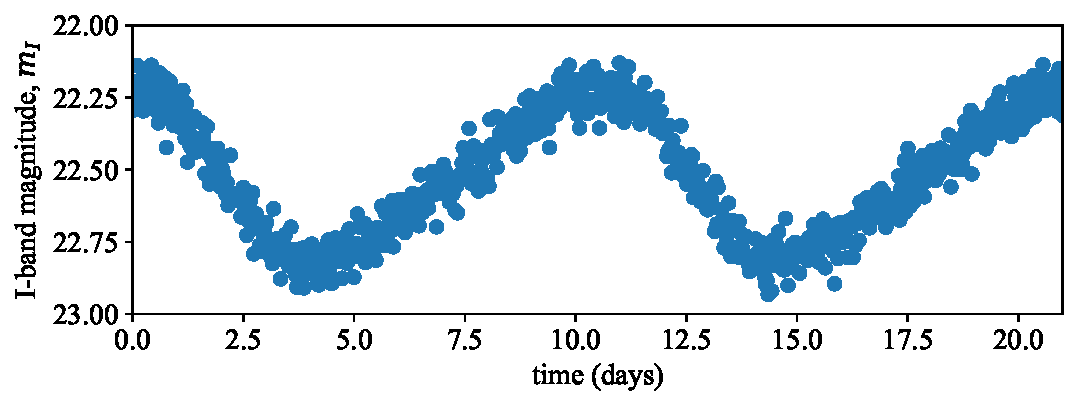
\includegraphics[width=0.7\textwidth]{exercises/distance_ladder/fake_cepheidII_800kpc.pdf}
  \end{center}
 
  
  % Detached eclipsing binaries

  % Maser

% II-p  
\item \label{ex:SNII-p} Work through an example of the expanding photosphere method for a Type II-p supernova, but consider the emission as a blackbody as a simplification.
  At time $t_1$, you measure shell 1 of the photosphere, and through photometry and spectroscopy you know that it has brightness $F_1$, constant velocity $v_1$,  and effective temperature $T_1$.  The unknown radius of the photosphere at that time is $r_1 = v_1 (t_1 - t_*)$, where $t_*$ is the unknown time of the explosion.  At time $t_2$, you similarly measure $F_2$, $v_2$, and $T_2$.
  \begin{enumerate}
  \item Argue that the ratio of the radii of the photospheres at $t_1$ and $t_2$ is
    $$
    \frac{r_1}{r_2} = \left( \frac{ F_1}{ F_2} \right)^{1/2} \frac{T_2^2}{T_1^2} = \frac{v_1}{v_2} \frac{t_1 - t_*}{t_2 - t_*} 
    $$
  \item Solve it to find $t_* = (t_1 - C t_2)/(1-C)$ where
    $$
    C = \frac{v_2}{v_1} \left( \frac{ F_1}{ F_2} \right)^{1/2} \frac{T_2^2}{T_1^2}
    $$
  \item What is then an expression for the luminosity distance $D_L$ in terms of $t_*$ and other quantities?

  \end{enumerate}
    This exercise is just to convince you that the measurement is feasible.  An actually application wouldn't solve for the distance but perform a multiparameter optimization to the (noisy) data, where $D_L$ is one of the parameters.
 
  
  
%
% at t1 we measure shell 1 which has radius r1 with v1, with r1 = v1*(t1 - t*)
% at t2 we measure shell 2 which has radius r2 with v2, with r2 = v2*(t2 - t*)
% F1 = sigma T1^4 r1^2 / DL^2
% F2 = sigma T2^4 r2^2 / DL^2
%
% r1/r2 = sqrt(F1 T2^4/ F2 T1^4) = v1/v2*(t1-t*)/(t2-t*)
%
%
% Solve for t* = ( t1 - C t2 ) / ( 1 - C )
%
% C = v2/v1 sqrt(F1/F2) T2^2/T1^2
%  
% Then F1 = sigma T1^4 (v1*(t1 - t*))^2 / DL^2
%
% DL = sqrt( F1 / (sigma T1^4 v1^2 (t1-t*)^2 ) )
%


  % GW siren
\item
  Consider the inspiral of a binary black hole system with two $50$ M$_\odot$ black holes (source frame) at redshift $z=2$.  Assume a flat $\Lambda CDM$ cosmology with $H_0 = 70$ km/s/Mpc and $\Omega_m = 0.3$ and an optimal, face-on inclination hitting an ideally oriented detector.
  
  \begin{enumerate}
    \item In Equation \ref{eqn:GW_distance_measure}, what factors of $G$ and $c$ restore the units of dimensionless strain $h = \delta \ell/\ell$.

    \item Calculate the chirp mass $\mathcal{M}_c$ and the detector frame chirp mass $(1+z)\mathcal{M}_c$.

    \item Determine the amplitude of the strain when the frequency passes through $50$ Hz (observed frame).

    \item Compute the strain noise amplitude spectral density (ASD) required to achieve a signal-to-noise (SNR) ratio of SNR=5 on the final 0.01s (observed frame) of the merger (you can unrealistically assume the frequency is constant.)

      Strain ASD has units of Hz$^{-1/2}$, and the required sensitivity can be computed as
      $$ \mbox{ASD} = \frac{h T^{1/2}}{SNR} $$
      where $T$ is the observation duration.

    \item Look up the sensitivity curves of the planned Einstein Telescope or Cosmic Explorer and compare.      
  \end{enumerate}
  
  % TRGB

  % Galaxy scaling relations

  % surface brightness fluctuations
\item  Think about surface brightness fluctuations in a galaxy at 10 Mpc, where a pixel of HST might contain 3000 stars. At this distance, the galaxy is larger than the field of view of the $4000 \times 4000$ pixel detector.  In the infrared, red giant stars dominate the emission, and at that distance have a brightness of about 15 nJy.  What pixel noise standard deviation can we tolerate to measure the brightness fluctuation flux to 1 percent considering the entire galaxy image?

  Realistically, HST will reach noise levels much lower than this, but the main sources of error are systematic: e.g. subtracting out globular clusters and background galaxies.



\end{enumerate}
